\documentclass[11pt]{article}
\usepackage{graphicx}
\usepackage{gensymb}
\begin{document}

\title{Simulation of Projectile Motion using Simulink}
\date{\today}
\maketitle

\section{Introduction}
This paper consists a simulation of a cricket ball undergoing projectile motion. It is given some initial velocity \textit{v} at an angle $\theta$ where the initial coordinates  are $(\textit{x}, \textit{y})= (0,0)$. Only the gravitational force acts on the body.

\section{Equations}
  Since there is no force acting in \textit{x} direction so by Newton's Equations of motion $$M\frac{d^2x}{dt^2} = 0\hspace{3cm}...(1)$$
  
There exists a gravitational force in negative \textit{y} direction of magnitude $Mg$, by Newton's Equations of motion $$M\frac{d^2y}{dt^2} =  -Mg\hspace{2.7cm}...(2)$$

\section{Simulink Diagram}
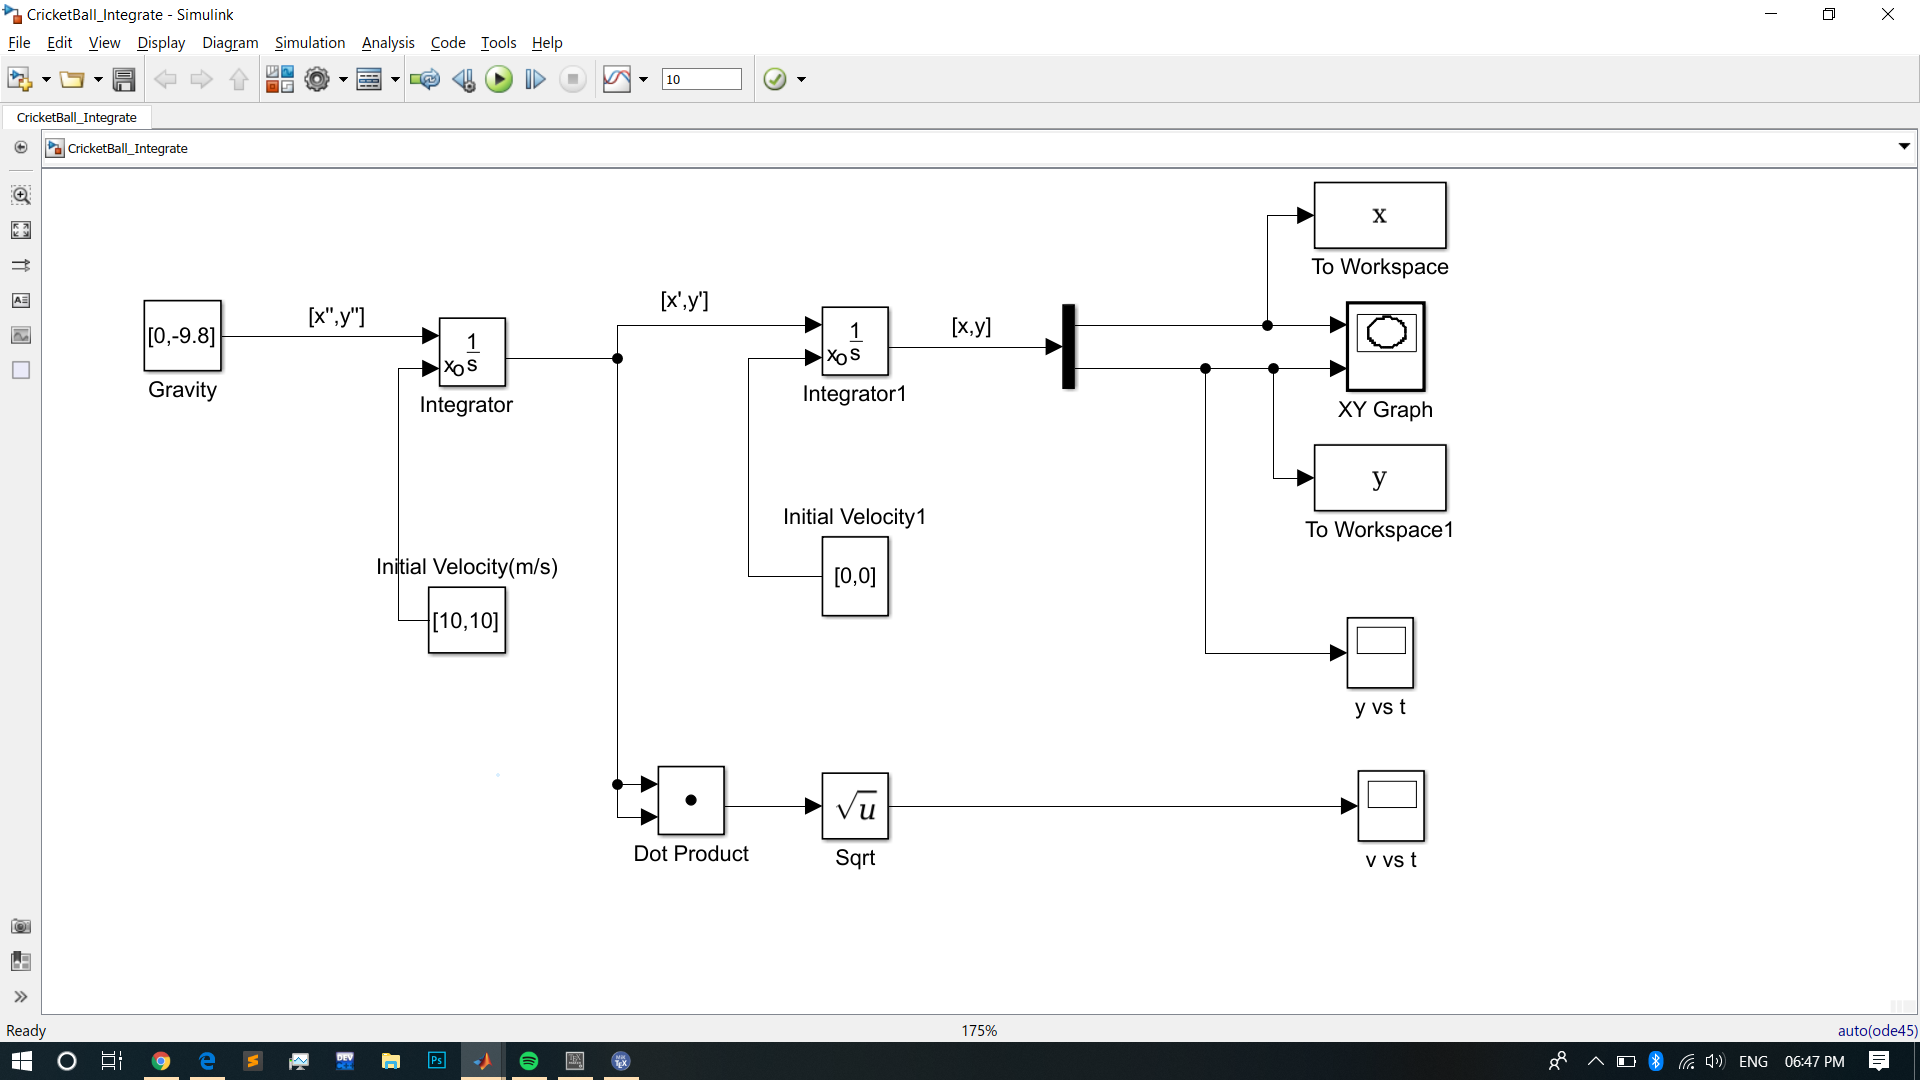
\includegraphics[scale=0.2]{Simulink_diagram.png} 
\subsection{Initial Conditions}
Initial velocity\hspace{1 cm}
$\textit{v}= 10\sqrt{2} m/s$\\
Angle of Projection\hspace{1 cm}
$\theta = 45\degree$\\
Initial Coordinates\hspace{1cm}
$x=0,\hspace{0.3cm}y=0$

\section{Integration Results}
\includegraphics[scale=0.2]{integration_results.png}\\ 
\\From Equations (1) and (2) we get,
$$x=u_{x}t$$
$$y=u_{y}t-\frac{1}{2}gt^2$$\\
where, $u_{x}$ and $u_{y}$ are horizontal and vertical component of Initial velocity $u$ respectively.

\section{Trajectory Figure}
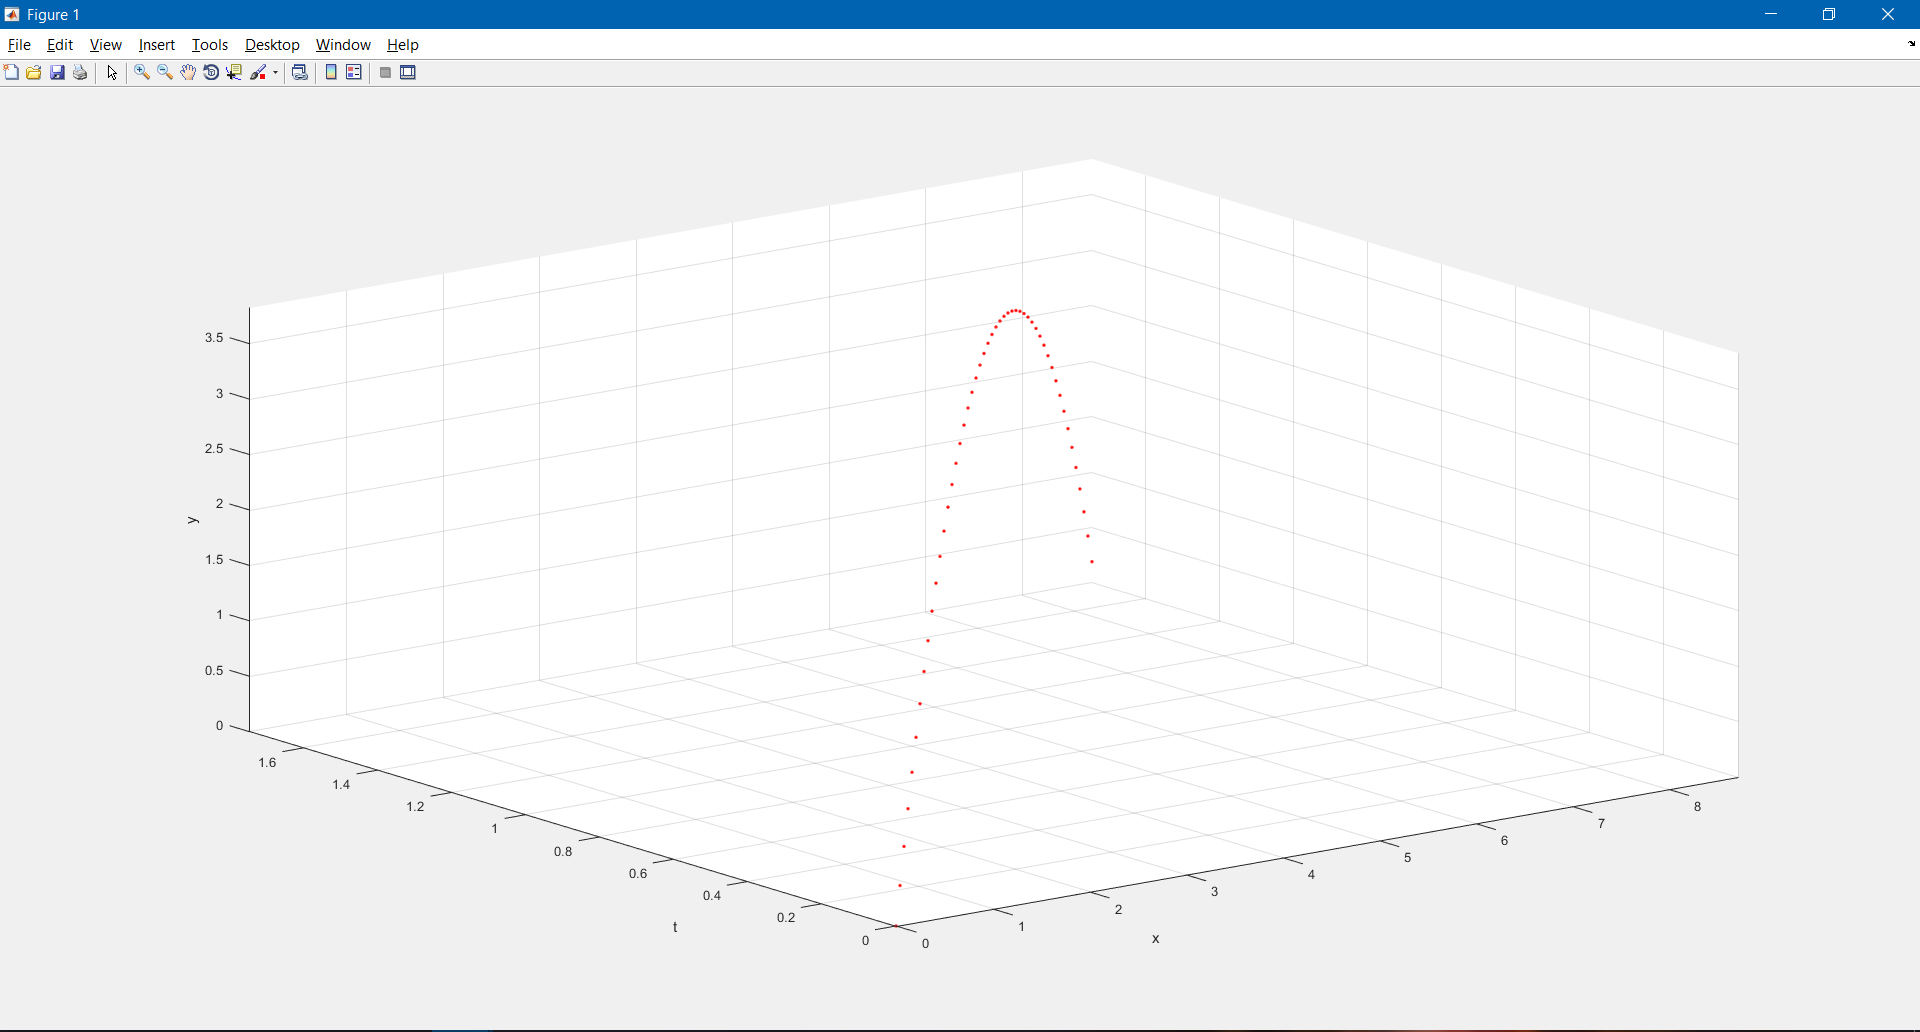
\includegraphics[scale=0.4]{Projectile.png} 
\end{document}